\documentclass[12pt, titlepage]{article}
\usepackage[utf8]{inputenc}
\usepackage{amsmath,amsthm,amsfonts,amssymb,amscd}
\usepackage{multirow,booktabs}
\usepackage[table]{xcolor}
\usepackage{fullpage}
\usepackage{lastpage}
\usepackage{enumitem}
\usepackage{fancyhdr}
\usepackage{mathrsfs}
\usepackage{wrapfig}
\usepackage{setspace}
\usepackage{calc}
\usepackage{multicol}
\usepackage{cancel}
\usepackage[retainorgcmds]{IEEEtrantools}
\usepackage[margin=3cm]{geometry}
\usepackage{amsmath}
\newlength{\tabcont}
\setlength{\parindent}{0.0in}
\setlength{\parskip}{0.05in}
\usepackage{empheq}
\usepackage{framed}
\usepackage[most]{tcolorbox}
\usepackage{xcolor}
\colorlet{shadecolor}{orange!15}
\parindent 0in
\parskip 12pt
\geometry{margin=1in, headsep=0.25in}
\theoremstyle{definition}
\newtheorem{defn}{Definition}
\newtheorem{reg}{Rule}
\newtheorem{exer}{Exercise}
\newtheorem{note}{Note}

\usepackage[superscript,biblabel]{cite}
\usepackage{hyperref}
\hypersetup{colorlinks,linkcolor={blue},citecolor={blue},urlcolor={orange}}

\usepackage{graphicx}
% Path relative to the main .tex file
\graphicspath{ {./images/} }

\title{\textbf{Practical integrator using operational amplifier}}
\author{
  Russel Shawn Dsouza\\
  171EC143
  \and
  Sathvik S Prabhu\\
  171EC146
}
\date{13 November 2019}

\begin{document}
  % TODO Add NITK logo
  % TODO Add 'AIC Report' and date
  \maketitle
  \thispagestyle{empty}

  \newpage
  \tableofcontents
  \thispagestyle{empty}

  \newpage
  \setcounter{page}{1}
  \section{Aim}
  To design, implement and test a $\mu$A741-based voltage integrator.


  \section*{Components required}
    \begin{itemize}
      \item $\mu$A741 OpAmp
      \item Resistors R = 120k$\Omega$, 3.3k$\Omega$, 4.7k$\Omega$
      \item Capacitor C = 0.01 $\mu$F
      \item Signal generator
      \item Digital Storage Oscilloscope
      \item Breadboard
      \item Jumper wires
    \end{itemize}


  \section*{Circuit diagram}
    % TODO Add circuit in LaTeX
    \begin{figure}
      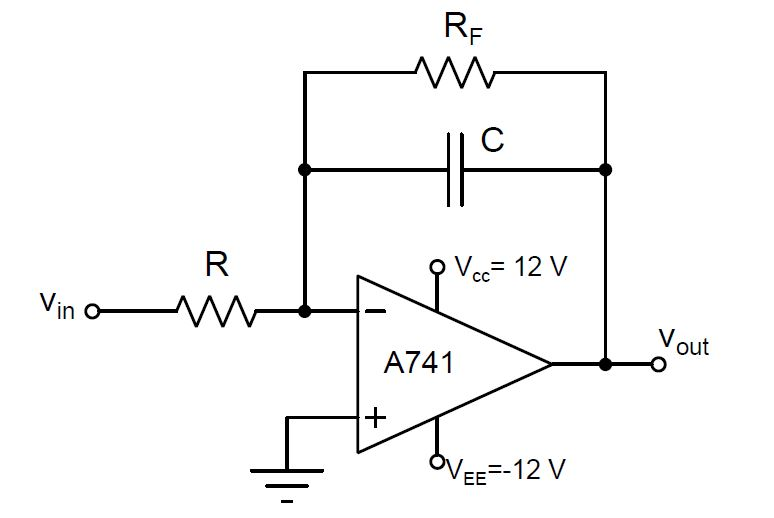
\includegraphics[scale=0.5]{circuit}
      \caption{Circuit diagram}
      \label{fig:theoretical_circuit}
    \end{figure}

    \begin{figure}
      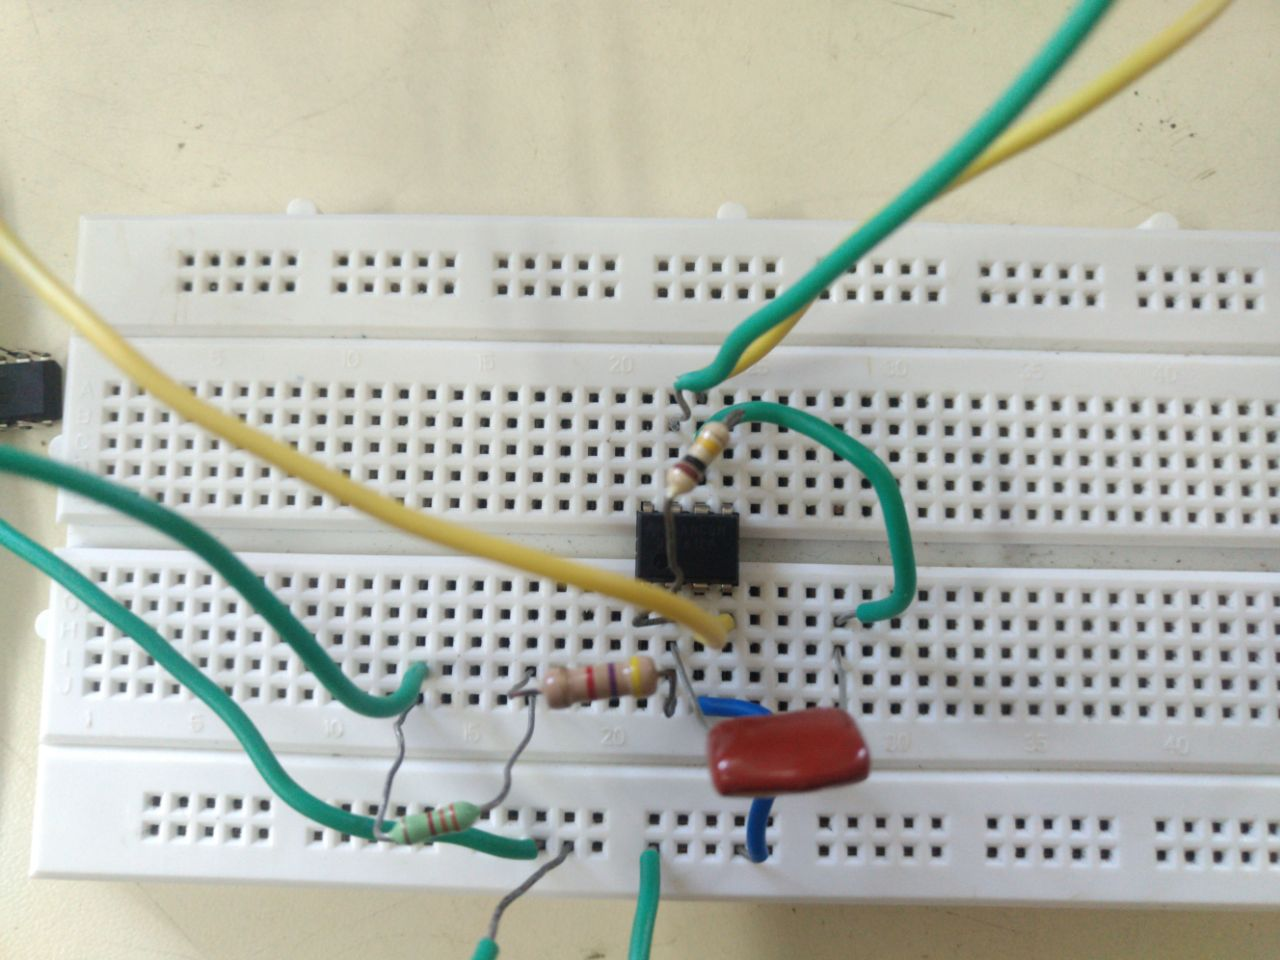
\includegraphics[scale=0.25]{practical_circuit}
      \caption{Designed circuit implemented on a breadboard}
      \label{fig:practical_circuit}
    \end{figure}

  \newpage
  \section{Theory}
    % TODO Complete Theory
    In an integrator, the output voltage is proportional to the integral of the input.
    The response of an opamp circuit with feedback will reflect the characteristics of the feedback elements.
    In order to achieve integration, the feedback network is constructed using a capacitor.

    In a practical integrator, one can overcome the limitations of an ideal integrator by adding resistor $R_{f}$ in parallel with capacitor $C$.
    $R_{f}$ prevents the opamp from going into open loop configuration at low frequencies.

    Frequency response of a practical integrator is given by,
    \begin{align}\label{eq:freq_response}
      H(s) &= \frac{-R_{F} || \frac{1}{Cs}}{R} \\
      H(j\omega) &= \frac{-R_{F}}{R} \left[ \frac{1}{1+R_{F}Cj\omega} \right]
    \end{align}

    The magnitude and phase response are given by,
    \begin{align*}
    |H(j\omega)| &= \frac{R_{F}}{R}\frac{1}{\sqrt{1+\omega^{2}R_{F}^{2}C^{2}}} \\
    \angle H(j\omega) &= \pi - tan^{-1}(\omega R_{F}C)
    \end{align*}

    \underline{DC gain} is obtained by putting $\omega = 0$ in equation\ref{eq:freq_response}.
    \begin{equation}
      DC gain = H(j0) = -\frac{R_f}{R}
    \end{equation}

    % TODO Add derivation
    \underline{Phase shift} is given by
    \begin{equation}\label{eq:phase_shift}
      \phi = \pi - \tan^{-1}(\omega R_FC)
    \end{equation}

    % TODO Add derivation
    \underline{$f_{-3dB}$} or cutoff-frequency is given by
    \begin{equation}\label{eq:f3db}
      f_{-3dB} = \frac{1}{2\pi R_FC}
    \end{equation}

    % TODO Add derivation
    \underline{$\omega_u$} or unity gain bandwidth is obtained from $|H(j\omega)| = 1$ giving,
    \begin{equation}\label{eq:unity_gain_bw}
      \omega_u = \frac{1}{RC}
    \end{equation}

    % TODO Add reason/derivation
    \underline{Roll-off rate} for the frequency response of the practical integrator is theoretically -20 $\frac{\text{dB}}{\text{decade}}$.

  \newpage
  \section{Design}
    % TODO Stepwise design
    Q. Design a $\mu$A741 based voltage integrator with unity gain and
    $f_{-3dB} = f_{in}/15$ for a sinusoidal input
    $v_{in} = 2 sin(4000\pi t)$, keeping the phase error below 5\%.
    \begin{align*}
        \text{Let C} \! &=0.01\mu F , \\
        f_{in} &=2000 Hz\\
        f_{-3dB} &=\frac{f_{in}}{15} = 133.33 Hz \\
        \frac{1}{2\pi R_{F}C} &= 133.33\\
        \frac{1}{2\pi RC} &= 2000\\
        R &=7.96k\Omega\\
        R_{F} &=119.37k\Omega\\
    \end{align*}


  \section{Calculations}
  % TODO Merge calculations with stepwise design
  \begin{align*}
    \text{Expected DC gain} &= \frac{R_{f}}{R}=15.25\\
    \text{Expected phase shift} &= \frac{\pi}{2}=1.57 rad
  \end{align*}


  \newpage
  \section{Simulation}
    % TODO Convert to white background images
    % TODO Add captions and labels
    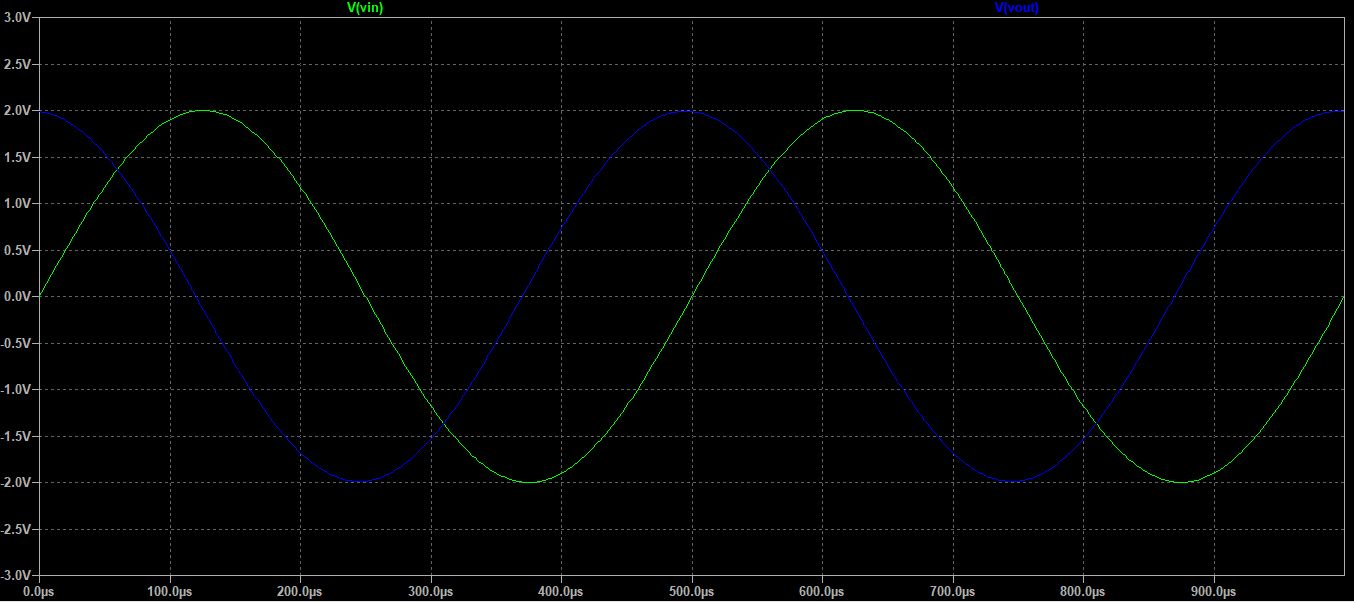
\includegraphics[width=\textwidth]{sim_plot1}
    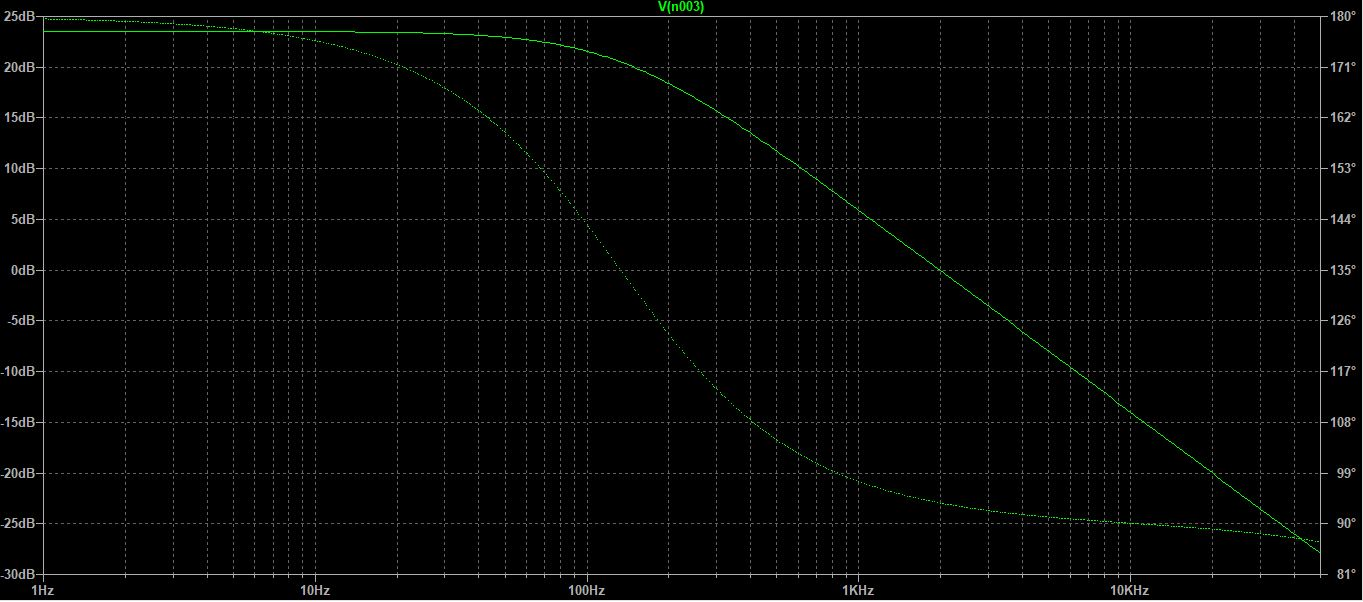
\includegraphics[width=\textwidth]{sim_plot2}


  \newpage
  \section{Waveforms}
    % TODO Add captions and labels
    \includegraphics[width=\textwidth/2]{results_q1}
    \includegraphics[width=\textwidth/2]{results_q3}
    \includegraphics[width=\textwidth/2]{results_q4_2}


  \newpage
  \section{Observations}
    \textbf{A}. The practical integrator is first designed based on the following constraints:
    Unity gain, $f_{-3dB} = f_{in}/15$ for a sinusoidal input
    $v_{in} = 2 sin(4000\pi t)$ and phase error below 5\%.

    A leading phase sinusoidal wave appears at the output of the integrator as shown in figure \ref{fig:results_q1}.
    The DC gain, -3dB frequency $f_{3dB}$, unity gain frequency $f_u$, roll-off rate and phase shift are noted from the waveforms obtained on the DSO and the phase error is verified to be below 5\%.

    \begin{figure}
      % TODO Add labels for Vin and Vout
      \includegraphics[scale=0.25]{images/results_q1.jpeg}
      \caption{Result of passing a sinusoidal input through the integrator}
      \label{fig:results_q1}
    \end{figure}

    % TODO Show calculation that was used to obtain these results
    \begin{itemize}
      \item[] DC gain = 14.89
      \item[] -3dB frequency = 132 Hz
      \item[] Unity gain frequency = 2.07 kHz
      \item[] Roll-off rate = -18.35 dB/decade
      \item[] Phase shift = 1.608 rad or $92.13^{\circ}$, an error of 2.4\%
    \end{itemize}


    \textbf{B}. The feedback resistor $R_F$ is then removed and the effect on the opamp integrator configuration is observed.

    \begin{figure}
      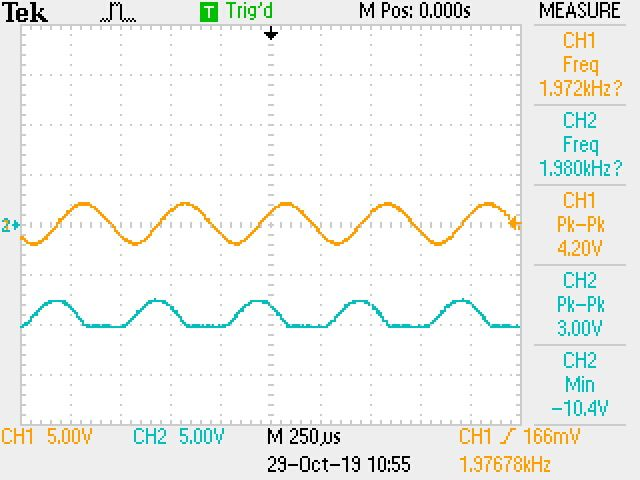
\includegraphics[scale=0.25]{images/results_q2.jpeg}
      \caption{The output of the integrator circuit without $R_F$}
      \label{fig:results_q2}
    \end{figure}

    The output is given by $V_{out}=\pm V_{sat}$ due to the capacitor acting as an open circuit at low frequencies as shown in figure \ref{fig:results_q2}.This sends the opamp into an open loop configuraton.


    \textbf{C}. The sinusoidal input is replaced by a square wave of 4$V_{pk-pk}$ amplitude and a frequency of 2kHz to observe the integration operation of the configuration more clearly.

    \begin{figure}
      % TODO Label Vin and Vout in figure
      \includegraphics[scale=0.25]{images/results_q3.jpeg}
      \caption{Result of integrating a square wave}
      \label{fig:results_q3}
    \end{figure}

    A triangular waveform is obtained as a result of the square wave being integrated, as shown in figure \ref{fig:results_q3}.

    $C\Delta V=I\Delta t$\\
    Substituting $C=0.01\mu F$, $I=\frac{2}{8k}$, $\Delta t=\frac{0.5}{2000}$, \\
    $\Delta V = 6.25 V$\\
    The output triangular waveform has a peak to peak voltage of around 6.25 V.

    D. The frequency of the input is lowered to 130Hz and the output is observed again on the DSO.

    \begin{figure}
      \includegraphics[scale=0.25]{images/results_q4_2.jpeg}
      \caption{Effect of lowering the input frequency on the output}
      \label{fig:results_q4}
    \end{figure}

    $C\Delta V=I\Delta t$\\
    Substituting $C=0.01\mu F$, $I=\frac{2}{8k}$, $\Delta t=\frac{0.5}{130}$, \\
    $\Delta V = 96.15 V$ \\
    Since $\Delta V > 2V_{sat}$, $V_{out}$ gets clipped as shown in figure \ref{fig:results_q4}.


  \newpage
  \section{Results \& Conclusions}
    % TODO Add more results and better conclusions
    The $\mu$A741 based voltage integrator was designed and implemented successfully.
\end{document}
